\documentclass[letter, 10pt]{article}
\usepackage[utf8]{inputenc}
\usepackage[spanish]{babel}
\usepackage{amsfonts}
\usepackage{amsmath}
\usepackage[dvips]{graphicx}
\usepackage{url}
%\usepackage[top=2cm,bottom=2cm,left=2.5cm,right=2cm,footskip=1.5cm,headheight=1.5cm,headsep=.5cm,textheight=3cm]{geometry}
\usepackage[top=3cm,bottom=3cm,left=2.5cm,right=2cm]{geometry}
\usepackage{listings}
\usepackage{color}
\usepackage{fancyvrb}
\usepackage{fancyhdr}

%%%%%%%%%%%%%%%%%%%%%%
%Estilo del documento%
%%%%%%%%%%%%%%%%%%%%%%
\pagestyle{fancyplain}

%%%%%%%%%%%%%%%%%%%%%%%%%%%%%%%%%%%%%%%%%%%
%Fancyheadings. Top y Bottom del documento%
%%%%%%%%%%%%%%%%%%%%%%%%%%%%%%%%%%%%%%%%%%%
% Recuerde que en este documento la portada del documento no posee
% numeracion, pero de igual manera llamaremos a esa primera pagina la numero
% 1, y la que viene la dos. Esto es para tener una idea de las que
% llamaremos pares e impares
\lhead{Comportamiento Organizacional} %Parte superior izquierda
\rhead{\bf \it Entrevista Apreciativa} %Parte superior derecha
\lfoot{} %Parte inferior izquierda.
\cfoot{} %Parte inferior central
\rfoot{\bf \thepage} %Parte inferior derecha
\renewcommand{\footrulewidth}{0.4pt} %Linea de separacion inferior


\begin{document}
\bibliographystyle{plain}

%%%%%%%%%%%%%%%%%%%%%%%%%%
%Definicion de la portada%
%%%%%%%%%%%%%%%%%%%%%%%%%%
\begin{titlepage}
    \begin{center}
	%\begin{tabular}{ccc}
	\begin{tabular}{c}
		
\includegraphics[width=0.9\textwidth]{img/logos}
		
	   % 
\includegraphics[width=3cm]{img/utfsm}
	   % & 
	   % \hspace{-0.2cm}
	   % \begin{tabular}{c}
	   % Universidad Técnica Federico Santa María \\ \hline
	   % \vspace{0.2cm}
	   % Departamento de Informática\\
	   % \vspace{1.2cm}
	   % \end{tabular}
	   % \hspace{0.2cm}
	   % &
        %    
\includegraphics[width=2cm]{img/di}
	\end{tabular}

	\vspace{4cm}
	%Titulo del Documento
	\begin{tabular}{c}
		\vspace{3cm}
		\Large{\sc{Seminario de Modelos y Métodos Cuantitativos}}\\
		\huge{\sc{Tarea 2}}\\\\
		%\includegraphics[scale=0.7]{img/portada} \\\\
	\end{tabular}

    \vspace{5cm}
	\begin{tabular}{lr}
			\textbf{Alumnos} & \\
							 & \\
         	\normalsize{Cristián Maureira Fredes} & \url{cmaureir@csrg.inf.utfsm.cl}\\
         	\normalsize{Gabriel Zamora Nelson} & \url{gzamora@csrg.inf.utfsm.cl}\\

							 & \\
			\textbf{Profesor} & \\
							 & \\
         	\normalsize{Andrés Moreira} & \url{amoreira@inf.utfsm.cl}\\
	\end{tabular}

\vspace{2cm}

	%Fecha
    \normalsize{\sc{\today}}\\
    %\normalsize \textbf{Fecha de Entrega:} & {14 de Noviembre del 2010}\\
    \end{center}
\end{titlepage}


\tableofcontents

\newpage
\section{Resumen}
%Explicar el contenido del trabajo en unas pocas líneas.
En el presente trabajo se realiza un análisis apreciativo a una organización en particular,
Ellian y Cia Ltda. para buscar características que nos indiquen el funcionamiento de la misma,
pero más importante aún experimentar al realizar preguntas positivas a distintos miembros de la
organización para buscar patrones y reacciones ante esta situación.


\section{Descripción de la Empresa}
%Nombre de la empresa, breve historia, organigrama, tipo de empresa,
%detalles de su funcionamiento, etc.

\subsection{Elian Y Cía., Ltda.}

Esta micro-empresa se encarga de la producción, venta y reparaciones de joyas, lleva más de veinte años en
la Quinta Región. Dispone de talleres propios siguiendo procesos a cargo de orfebres especializados.
Elaboran todo tipo de cadenas, anillos, argollas de matrimonio y colgantes (de oro y plata).
Se han preocupado por implementar nuevas tecnologías, ofreciendo fotograbado a color en Plata, Oro y
Acero.

Posee 4 sucursales de ventas y una casa central donde tienen todo el proceso de producción. El personal
no son más de 30 personas, es una organización exigente, pero preocupada por el bienestar de sus
trabajadores. Como se manejan objetos pequeños de gran valor, la confianza en los trabajadores y buenos
métodos de control son primordiales para la empresa. Por ello, el ambiente entre los colaboradores es muy
familiar, donde la alta gerencia está conformada por el jefe de todos, Sr. Iván González y el gerente de
ventas y producción, su hijo Iván González.

Las áreas de trabajo en la empresa se pueden identificar como
ventas (vendedores de cada sucursal), producción (la mayoría orfebres) y administración (secretarias, 
informática y gerencia).


\section{Breve descripción del proceso de aplicación de la entrevista}
%¿Cuántas personas fueron entrevistadas?, ¿cuándo?, ¿cómo?, ¿se dieron
%facilidades para la toma de entrevistas?, ¿qué se observó durante el
%proceso?, etc.

Fueron entrevistadas 10 personas de la empresa. Para ello se realizaron 2
visitas los días 1 y 6 de Septiembre. Éstas se realizaron individualmente, en
una sala privada, en presencia de los 3 integrantes del equipo, a excepción de
algunas que tuvieron que realizarse en las sucursales de venta de la empresa,
en donde se tuvo que realizar en el mismo lugar donde trabajan las vendedoras.

Se observo una evolución positiva durante la realización de la encuesta por
parte de los entrevistados, en donde en su mayoría lograron abrirse y contar
experiencias que no se limitaban a las preguntas que nosotros realizábamos.
También se logró identificar un efecto de desahogo y alivio al terminar la
entrevista. Un caso inclusive nos agradeció haberlo entrevistado.

La persona a cargo de la organización tuvo una muy buena disposición al permitirnos
entrevistar a cualquier persona y poder acceder a las instalaciones de la empresa.

Las entrevistas en los talleres tenían un toque más personal, pues se estaba en una
sala cerrada, donde nadie escuchaba o transitaba, por lo que las personas se sentían más
en confianza, lamentablemente en los centros de ventas no fue así puesto que constantemente
entraban clientes y se tenía que interrumpir la entrevista, lo cual en nuestra opinión
no permitía abrirse completamente a las vendedoras, pero aún así hicieron lo mejor que pudieron.


\section{Entrevista Apreciativa}
%Transcribir las preguntas que conformaron su entrevista
%(no las
%respuestas). Estas preguntas deberán incorporar las posibles correcciones
%realizadas por los ayudantes luego de la entrega de la parte 1.
\begin{enumerate}
    \item  ¿Qué significa para ti pertenecer a esta organización? 
    \item  ¿Cuáles han sido los mejores logros/aportes que has realizado?
    \item  ¿Cuál es la meta que más te motiva al trabajar?
    \item  ¿De qué forma mejorarías algo que ya es bueno dentro de tu organización?
    \item  ¿Te gustaría poder ejercer más tu creatividad en el trabajo?
    \item  ¿Cuales crees tú que son los logros de la organización?
    \item  ¿Qué es lo mejor de tu grupo de trabajo?
    \item  ¿Cuál es la actividad dentro de tu organización que más te ha gustado?
    \item  ¿Quién es el mejor elemento dentro de la empresa según tu opinión? ¿Porqué?
    \item  ¿Qué momento del día/semana es tu favorito? ¿Por qué?
    \item  ¿Como te vez en la organización en 5 años más?
    \item  ¿De quién te sientes más agradecido dentro de la organización?
    \item  Si pudieras volver al momento en que decidiste trabajar acá, ¿volverías a aceptarlo? ¿Por qué?
    \item  ¿Qué te gustaría que se recordara de ti cuando te vayas?
    \item  ¿Qué elemento de motivación te gustaría crear dentro de la empresa?
\end{enumerate}


\section{Análisis de la aplicación de la entrevista}
% Análisis de la Aplicación de la Entrevista. (30%)
% Este análisis constituye la parte esencial del informe. Debe incluir:
%  Citar principios de la Entrevista Apreciativa aplicados u
% observados.
%  Se deben analizar las encuestas realizadas citando a los
% entrevistados para apoyar el análisis. También debe incorporar las
% observaciones que haya hecho in situ.
%  Explicitar los elementos descubiertos a través de la actividad
% (entorno de la organización, recursos, funcionamiento, etc.).


La mayoría de los entrevistados sentían que el mejor día de la semana era
cuando salían del trabajo, y podían realizar otras actividades recreativas o
con su familia.

Todavía se sentía la pérdida de un compañero de trabajo que habían despedido
hace 3 años atrás.

Con respecto al entorno de trabajo, pudimos percatarnos que existía un marcado
exceso en las horas de trabajo, lo que provocaba malestar e indiferencia en los trabajadores,
más lo que podría ser una presión social por parte de la dirección a que esta se
mantuviera (sin pagar las horas extras).

Por lo general, no existían problemas con los pagos de las cotizaciones, y todos los trámites
estaban al día, además no hubo ninguna queja con que faltara algún implemento para el trabajo
ya que para el almuerzo, se tiene un refrigerador, microondas, cada taller tiene una radio e
incluso algunos tienen un televisor, por lo que el ambiente es grato con respecto a elementos
tecnológicos que puedan necesitar.

Algunas actividades (salidas de fin de año, actividades en conjunto con todos
los empleados) que se realizaban en la empresa, se dejaron de desarrollar
hace unos 2 o 3 años atrás, y a todos les gustaría volver a ellas, o realizar
actividades nuevas que integren a todos como equipo.

Se ve al Jefe como a una figura paterna. Unas veces preocupado por sus
empleados, y otras veces como, citando a un entrevistado "dictador", lo cual
significa dos cosas, quizás problemas personales entre el Jefe y el entrevistado,

Algunos entrevistados se referían "al grupo en general", y utilizaban frases como
"son preocupados" pero otros se referían diciendo "cada uno mata su chancho",
lo que a pesar de no ser tantos trabajadores, nos muestra que tenemos los dos lados
de la moneda, personas que tienen un sentimiento negativo con el jefe por los malos
tratos y otros que dicen estar felices, aunque pueden ser de las personas que solo
bajan la cabeza y aceptan lo que el jefe diga, independiente que sea justo o no.

Una pregunta realizada, que se relaciona directamente con uno de los principios de la
entrevista apreciativa\cite{apreciativa} que nos dice "lo que se hace bien se puede hacer mejor",
descolocaba a las personas y pocos entrevistados pudieron realmente responderla,
ya que cuando les decíamos que si pudieran mejorar algún aspecto positivo, que harían,
nos respondían de inmediato que no podían y nosotros insistíamos que era un caso
hipotético y se desviaban del tema o nos señalaban que sería bueno agregar algún otro
elemento, pero las pocas personas que nos referíamos anteriormente, señalaron que 
quizás el ambiente sería mucho mejor con más actividades que unieran al grupo de trabajo.

Otra de las características importantes en la organización es que lamentablemente absolutamente
todos los trabajadores tienen la idea de que sin el Jefe, la empresa no va a funcionar, lo cual
es un aspecto negativo pues el Jefe está viejo y de a poco sus hijos han ido tomando el control
de la organización, a lo que los trabajadores no se contentan del todo.

Otro principio que se presenta en la entrevista, es el principio "principio anticipatorio", el cual 
esencialmente afirma que las imágenes del futuro pueden afecta la manera como nos comportamos en el presente. 
En particular, si tenemos una imagen particularmente deseable del futuro es muy probable que nos conduzcamos 
de maneras que lo cristalizarán. Es exactamente lo que se ve en algunos entrevistados, los cuales se veían
mas fuera de la empresa que dentro, por lo que su forma de describir su estado actual dentro de élla, demostraba
en gran medida lo que deseaban para su futuro.

Finalmente, la organización funciona sin problemas, aunque varios trabajadores les gustaría un poco
más de motivación, aumentos de sueldos o por último que se cumplieran los horarios.

% escribir mas


\section{Plan de Acción Propuesto}
%Diseño de un plan de acción con propuestas para el futuro de la empresa, de
%acuerdo a lo analizado.

De acuerdo a lo analizado en los puntos anteriores, claramente se ve una 
cierta disconformidad en las personas que se desenvuelven en esta empresa,
por lo que hay que tener presente que en el normal funcionamiento, es 
fundamental establecer un ambiente acorde a ello, ya sea físico como
psicológico. Para poder establecer dicho objetivo, planteamos lo siguiente:

% Esto está demasiado VERDE!!!! agreguen o modifiquen cosas (gzamora)

% De administracion general:
%1.-PREVISION
%2.-PLANEACION
%3.-ORGANIZACION
%4.-INTEGRACION
%5.-DIRECCION
%6.-CONTROL

\begin{itemize}
	\item Prever problemas. \\
	Se debe claramente prever los problemas que actualmente se han
	detectado dentro de la empresa. Para dicho propósito, se debe detectar las causas
	que provocan dichos problemas, con tal de mitigar aquello.
	Sería muy positivo, poder constar con algún mecanismo donde se puedan conversar
	todas las situaciones que ocurren en la empresa, como por ejemplo
	reuniones cada 2 semanas (se explica más adelante) donde todos puedan
	tocar algún tema determinado y aclarar todo, de ésta forma se pueden prever
	futuros conflictos. 

	\item Planear soluciones. \\
	La planeación de las soluciones va de la mano con actividades en las cuales todos puedan dar
	a conocer su opinión con respecto a una temática en particular, es necesario que la dirección
	de la organización no haga oídos sordos a éstas inquietudes, para poder mejorar el ambiente
	y el bienestar de cada miembro de la organización.
	Se tiene muy claro que no se le puede dar \emph{todo} lo que los trabajadores quieran, pero es
	necesario conversar las cosas y llegar a un acuerdo.

    \item Mejorar la organización.\\
	Actualmente existe una clara preferencia a las gestiones del Jefe, y se le ve como un
	elemento fundamental para que la organización funcione, hay que buscar con urgencia que
	no exista tal dependencia, puesto que la estadía del Jefe no es eterna, y por lo apreciado
	en las entrevistas, va a ser muy difícil el día que no esté para la organización seguir
	en igual funcionamiento como lo ha hecho hasta el momento. Es necesario más integrar y hacer
	que se simpatice con los futuros encargados, como en éste caso son los hijos.

	\item Actividades de integración.\\
	Variadas personas se referían a los momentos en que todos estaban unidos, como los buenos
	momentos de la organización, si bien es cierto algunas personas realmente no disfrutan de estar
	en grupo, es válido crear instancias más constantes, como por ejemplo, si se le van a celebrar los cumpleaños
	a los trabajadores, que sean a \emph{todos} y no sólo cuando el jefe dé la
    autorización\cite{integracion}.
	De la misma forma, sería recomendable retomar los paseos de fin de año para que todos los trabajadores se
	logren unir más.
	Finalmente, varios trabajadores se veían muy interesados en poder participar de charlas sobre distintas
	temáticas de actualidad para poder nutrirse de conocimiento y estar al día con respecto a un tema en particular,
	ya que nos plantearon las ganas de aprender cosas nuevas, no necesariamente relacionadas con la joyería.
	
	\item Aspectos de la dirección de la organización. \\
	La dirección de la organización se ha realizado de buena forma, pues ha tenido un crecimiento sustancial desde
	su comienzo, por lo que se percibe el esfuerzo detrás, pero hay que tener en cuenta que se deben cumplir
	las leyes del trabajo al pie de la letra, si bien es cierto hay mucho trabajo algunos días, los trabajadores
	están en todo su derecho para poder trabajar las horas que les corresponde, y si llegan trabajar horas extras
	estas deben ser remuneradas.
	
	\item Control de cada elemento de la organización. \\
	Actualmente no existe un control de cada miembro de la organización, aparte de que el Jefe algunas veces
	se acerca a las personas a preguntar como están.
	Sería muy recomendable que existiera una persona dedicada a analizar el comportamiento de cada miembro,
	quizás un especialista como un asesor externo, para poder estudiar a cada persona con lo cual se puede
	justificar quizás un bajo desempeño y al buscar la solución, poder tener a un personal trabajando cómodamente,
	sabiendo que se preocupan de sus problemas y con lo mismo la productividad de la organización se verá en aumento.

	% ESTO NO ES DE LA LISTA ORIGINAL PROPUESTA POR gzamora.

    \item Mejorar sistema de incentivos.\\
    Actualmente, los trabajadores no se sienten motivados~\cite{motivacion} a innovar y ser más
    creativos en su trabajo~\cite{creatividad}. Esto puede que se vea como algo positivo en
    cuanto se siguen las reglas impuestas al pie de la letra, pero se
    transforma en una fuente de disconformidad laboral al hacer más monótona
    la actividad diaria. Se recomienda tomar en consideración este punto, y
    generar un sistema de incentivos bien definido y que de verdad sienta en
    las personas que su trabajo y creatividad personal es reconocido.\\

    \item Plan de crecimiento personal.\\
    Estando trabajando muchos años en una misma empresa, logra especializar a
    las personas en lo que hace, lo cual es bueno en un comienzo, pero que
    hace que la persona deje de aprender cosas nuevas y sienta la inquietud de
    tener nuevas experiencias y aprender cosas nuevas. La idea es mantener el
    interés de las personas por su trabajo\cite{interes}, dándoles la oportunidad de poder
    perfeccionarse y/o aprender cosas nuevas complementarias a su área de
    trabajo. Ésto se puede realizar a través de pequeños cursos,
    capacitaciones o charlas libres para ciertos empleados de la empresa.

    \item Reuniones periódicas.\\
    Se recomienda realizar reuniones que den la libertad de
    discutir temas concernientes a las dinámicas internas de la empresa,
    problemas entre los miembros del personal o disconformidades varias que
    puedan tener, en donde se busque proponer los problemas y la solución a
    ellos, discutiendo todos de par-a-par dejando de lado por un momento los
    rangos de cada uno. Para ello se recomienda utilizar dinámicas de grupo
    focal (focus group~\cite{Grupo_focal}), con un moderador imparcial que
    controle que las conversaciones no se vallan por otros temas y den un
    orden a la actividad.

\end{itemize}

\newpage

\section{Conclusiones individuales}
%Cada alumno se debe identificar y dar una conclusión personal acerca de los
%temas tratados.

\begin{itemize}
	\item Rodrigo Fernández\\ \\
        Es bastante complejo el lograr reacciones positivas a diferentes
        personas bajo un sólo cuestionario en común, ya que las experiencias de
        diferentes grupos de personas condicionan de diferente forma la
        emotividad de cada una. Aún así, considero que la encuesta fue exitosa, ya
        que nos permitió identificar claramente la situación actual de la
        empresa, los puntos positivos que la hacen mantenerse con éxito, y las
        problemáticas que ha tenido a través del tiempo y que se pueden mejorar.
        Tomando en consideración la actividad realizada anteriormente con la
        empresa, este tipo de entrevista logró identificar y sacar a relucir a
        más detalle el estado actual de la organización, junto con las
        fortalezas, debilidades y posibles amenazas que pudieran afectarle en
        un futuro.
        Por último, el tema de las relaciones interpersonales dentro de los
        grupos de trabajo se logró destacar como un factor importante a la
        hora de evaluar la satisfacción de los trabajadores con su trabajo, y
        es posible que, como dicen algunos estudios, esté intrínsecamente
        relacionado con el desempeño laboral.
	\item Cristián Maureira \\ \\
		Al momento de redactar la entrevista, fue más difícil de lo habitual
	poder escribir las preguntas, porque realmente nos dimos cuenta que por lo
	general no pensamos "apreciativamente".
	Con respecto a los entrevistados, la experiencia fue muy similar a la que
	ya habíamos realizado en el ramo anterior, pero me pareció muy llamativo
	que a las personas les costaba mucho o simplemente no podían responder
	algunas preguntas, ya que no entendían lo que había que responder, como
	por ejemplo ¿Qué sientes al trabajar acá?, nos preguntaban a que nos
	referíamos y que diéramos un ejemplo, quizás las personas no están acostumbradas
	a responder preguntas de como se sienten o que consten en buscar entre sus
	propios logros.
	Finalmente comprobé lo que el profesor decía en clases acerca de que depende
	de la forma en que uno pregunta las cosas, puede interferir en lo que se responde,
	por ejemplo, malamente en varias ocasiones, preguntaba, ¿Pero usted se siente cómoda
	con su grupo de trabajo, no es cierto? y me decían "sí, por supuesto".

	\item Gabriel Zamora \\ \\
		La forma en que influyó el método apreciativo que tratamos de ejercer
	sobre los entrevistados, en cierta medida resulto bastante bien, ya que 
	algunos pocos se sentían bastante bien trabajando en aquel lugar. Sin
	embargo, una gran mayoría estaba predispuesta a responder en forma de
	demostrar su malestar sobre ciertas condiciones laborales, incluso 
	demostrándolo con sus gestos, lo que provocó que sus respuestas fueran
	bastante poco explicativas y de aspecto negativo, logrando finalmente
	que la entrevista fuera casi una queja a un tercero, para que se le 
	hiciera llegar a su jefe. Creo que a pesar de ésto último, se logró
	sacar ciertas cosas positivas en las respuestas y entre los pocos que 
	respondían positivamente, logramos sacar ideas escondidas que un cierto
	grupo poseía, como el hecho de independizarse o buscar un trabajo que le
	ofrezca mejores condiciones.


\end{itemize}


\newpage

\section{Conclusiones generales}
%Conclusión elaborada por todos los miembros del equipo en conjunto.

La experiencia fue muy enriquecedora al poder comprobar la reacción de las personas
al enfrentarse a una entrevista apreciativa, era fácil pode ver cuando se hacían sonrisas
en sus rostros y no había una tensión que empañara la entrevista, no había tensión al responder,
la gente lo paso muy bien y no fue como la entrevista pasada, donde algunos rostros quedaron
serios.

Algo muy importante que quedó muy en claro en el trabajo, es que muy pocas personas
tienen una autoestima alta que les permita decir "si, soy bueno en lo que hago",
ya que por otro lado hay personas que simplemente no podían decir ningún logro personal.

La organización escogida, no posee tantos trabajadores, por lo que se pudo comprobar el buen ambiente
que existía entre los trabajadores de las distintas áreas, sin dejar de lado algunos conflictos entre
un par de personas, que provocaban indiferencia, pero no un mayor conflicto.
Los espacios para almorzar juntos, por ejemplo, están pero no todas las personas se dan el tiempo
de almorzar en grupo, algunos almuerzan en su mismo lugar de trabajo, lo que hace alejarse más
la posibilidad de tener un gran equipo de trabajo.

Existen muy generalmente dos perfiles de trabajadores en la organización, aquellos que sólo acatan
todo lo que se les dice, y aquellos que están muy pendiente de si son pasados a llevar en sus
derechos, por ejemplo con el tema de las sobre-horas de trabajos, algunos se referían con rabi a la
situación y otros sólo decían que era necesario por la pega.

Además, hay ciertas figuras en la empresa, aparte del Jefe, que son de vital importancia para algunas
personas. Por ejemplo en el taller, existe una mujer que la mayoría ve casi como una madre y le
agradece por toda la preocupación, y por otro lado en las salas de ventas, las vendedoras han construido
una relación más de amistad que sólo de compañeras de trabajo, lo cual es positivo ya que el ambiente
es mucho más cálido al llegar a cualquier local y por lo menos al realizar las entrevistas así lo notamos.

Finalmente, pese a todos los problemas, pensamos que éste grupo de trabajo puede llegar a convertirse
en un equipo con un poco de esfuerzo de cada uno y algunas nuevas medidas realizadas por el jefe para
aumentar el bienestar de sus trabajadores.

\newpage

\section{Referencias}
\bibliography{referencias}
\newpage

\section{Anexos}
% Agregar:
% antecedentes recolectados
% otros (imágenes, textos, tablas, etc.)




\subsection{Actividades y tiempos empleados por cada integrante}

\begin{tabular}{|l|p{7cm}|c|}
\hline
Integrante & Actividades & Tiempo Empleado \\\hline
Cristián Maureira & Observación de los medios de comunicación y reuniones internacionales. & 7 horas \\
& Creación del Repositorio de trabajo. & 30 minutos \\
& Creación del esqueleto del informe.& 30 minutos \\
& Desarrollo de la introducción. & 2.5 horas \\
& Redacción de los análisis y resultados de antecedentes. & 3 horas \\
& Revisión de los análisis y resultados de antecedentes. & 1 hora \\
\hline
Gabriel Zamora & Revisión de  las formas de trabajo de cada grupo. & 8 horas \\
& Estudio del público objetivo y del dominio del trabajo. & 3 horas \\
& Redacción de los análisis y resultados de antecedentes. & 4 horas \\
\hline
Rodrigo Fernández & Comparación de los resultados con los antecedentes
recopilados. & 5 horas \\
& Investigación de la información existente. & 5 horas \\
& Redacción de los análisis y resultados de antecedentes. & 3 horas \\
& Revisión del análisis y resultados de antecedentes. & 30 minutos \\
& Revisión ortográfica del informe. & 10 minutos \\
\hline
\end{tabular}
\newpage
\subsection{Participantes de las reuniones}
\subsubsection{OSF Coordination Meeting}

\begin{tabular}{|l|l|l|l|}
	\hline
	{\bf Nombre} & {\bf Cargo} & {\bf Organización} & {\bf País} \\\hline
	Heiko Sommers & ACS Technical Leader & ESO & Alemania \\\hline
	Gianluca Chiozzi & ESO Astronomical Instrumentation Leader & ESO & Italia \\\hline
	Alessandro Caproni & Software Engineer& ESO & Italia \\\hline
	Matias Mora & Software Engineer & ALMA & Chile \\\hline
	Nicolas Troncoso & Software Engineer & ALMA & Chile \\\hline
	Jorge Avarias & Software Engineer & NRAO & EEUU \\\hline
	Rodrigo Tobar & Software Engineer & ESO & Alemania \\\hline
	Jaime Pavlich & Profesor & UCN & Chile \\\hline
	Tomas Staig & Computer Science Student & UTFSM/ESO & Chile \\\hline
	Arturo Hoffstadt & Computer Science Engineer & UTFSM/NRAO & Chile \\\hline
	Gabriel Zamora & Computer SCience Student & UTFSM & Chile \\\hline
	Cristián Maureira & Computer SCience Student & UTFSM & Chile \\\hline	
\end{tabular}

\subsubsection{ACS Weekly Meeting}

\begin{tabular}{|l|l|l|l|}
	\hline
	{\bf Nombre} & {\bf Cargo} & {\bf Organización} & {\bf País} \\\hline
	Joseph Schwarz & ACS Project Leader & ESO & Alemania \\\hline
	Heiko Sommers & ACS Technical Leader & ESO & Alemania \\\hline
	Gianluca Chiozzi & ESO Astronomical Instrumentation Leader & ESO & Italia \\\hline
	Alessandro Caproni & Software Engineer& ESO & Italia \\\hline
	Jorge Avarias & Software Engineer & NRAO & EEUU \\\hline
	Rodrigo Tobar & Software Engineer & ESO & Alemania \\\hline
	Arne Grimstrup & Software Engineer & NRAO & Canada \\\hline
	Bogdam Jeram & Software Engineer & ESO & Eslovenia \\\hline
	Helmut Tischer & Software Engineer & ESO & Alemania \\\hline
	Matej Sekoranja & Software Engineer  & ESO & Eslovenia \\\hline
	Roberto Cirami & Software Engineer & INAF - OAT & Italia\\\hline
	Tomas Staig & Computer Science Student & UTFSM/ESO & Chile \\\hline
	Gabriel Zamora & Computer Science Student & UTFSM & Chile \\\hline
	Cristián Maureira & Computer Science Student & UTFSM & Chile \\\hline	
\end{tabular}

% CORRECCION 6
\subsubsection{Fotografías}
A continuación se muestran algunas fotografías tomadas mientras se realizaban las reuniones semanales.\\

\begin{center} 
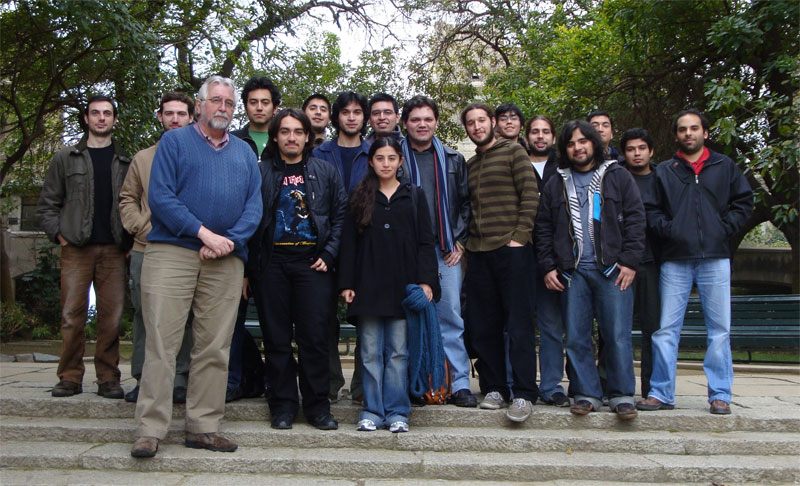
\includegraphics[width=0.8\textwidth]{images/alma-utfsm-1}\\\vspace{1cm}
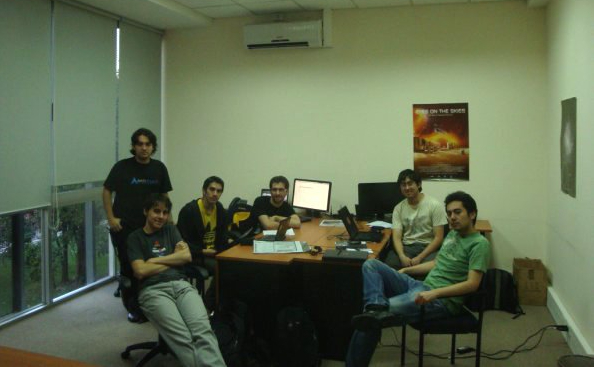
\includegraphics[width=0.8\textwidth]{images/alma-utfsm-2}\\
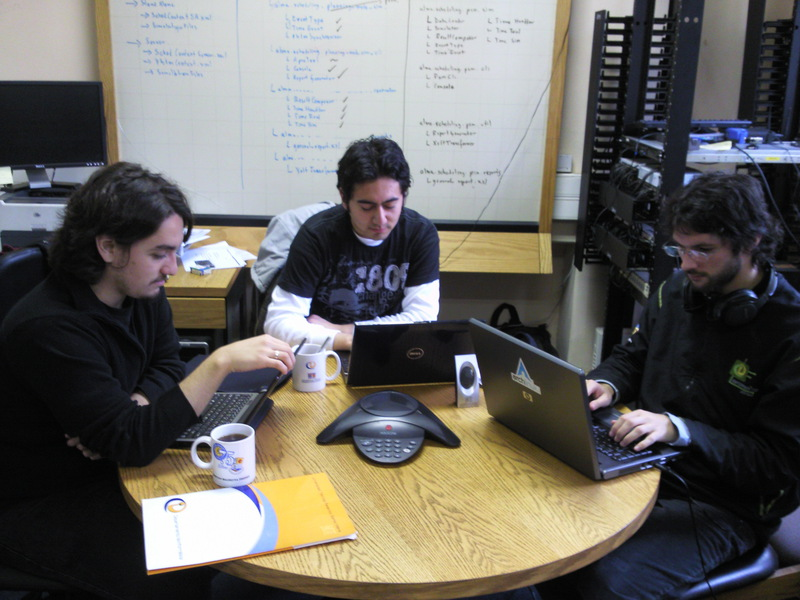
\includegraphics[width=0.8\textwidth]{images/lab_conference}\\\vspace{1cm}
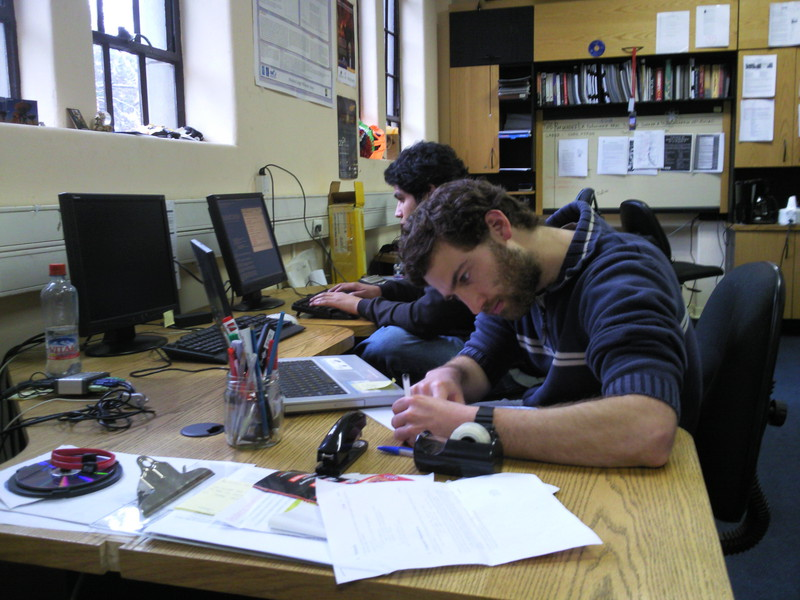
\includegraphics[width=0.8\textwidth]{images/lab_working}\\
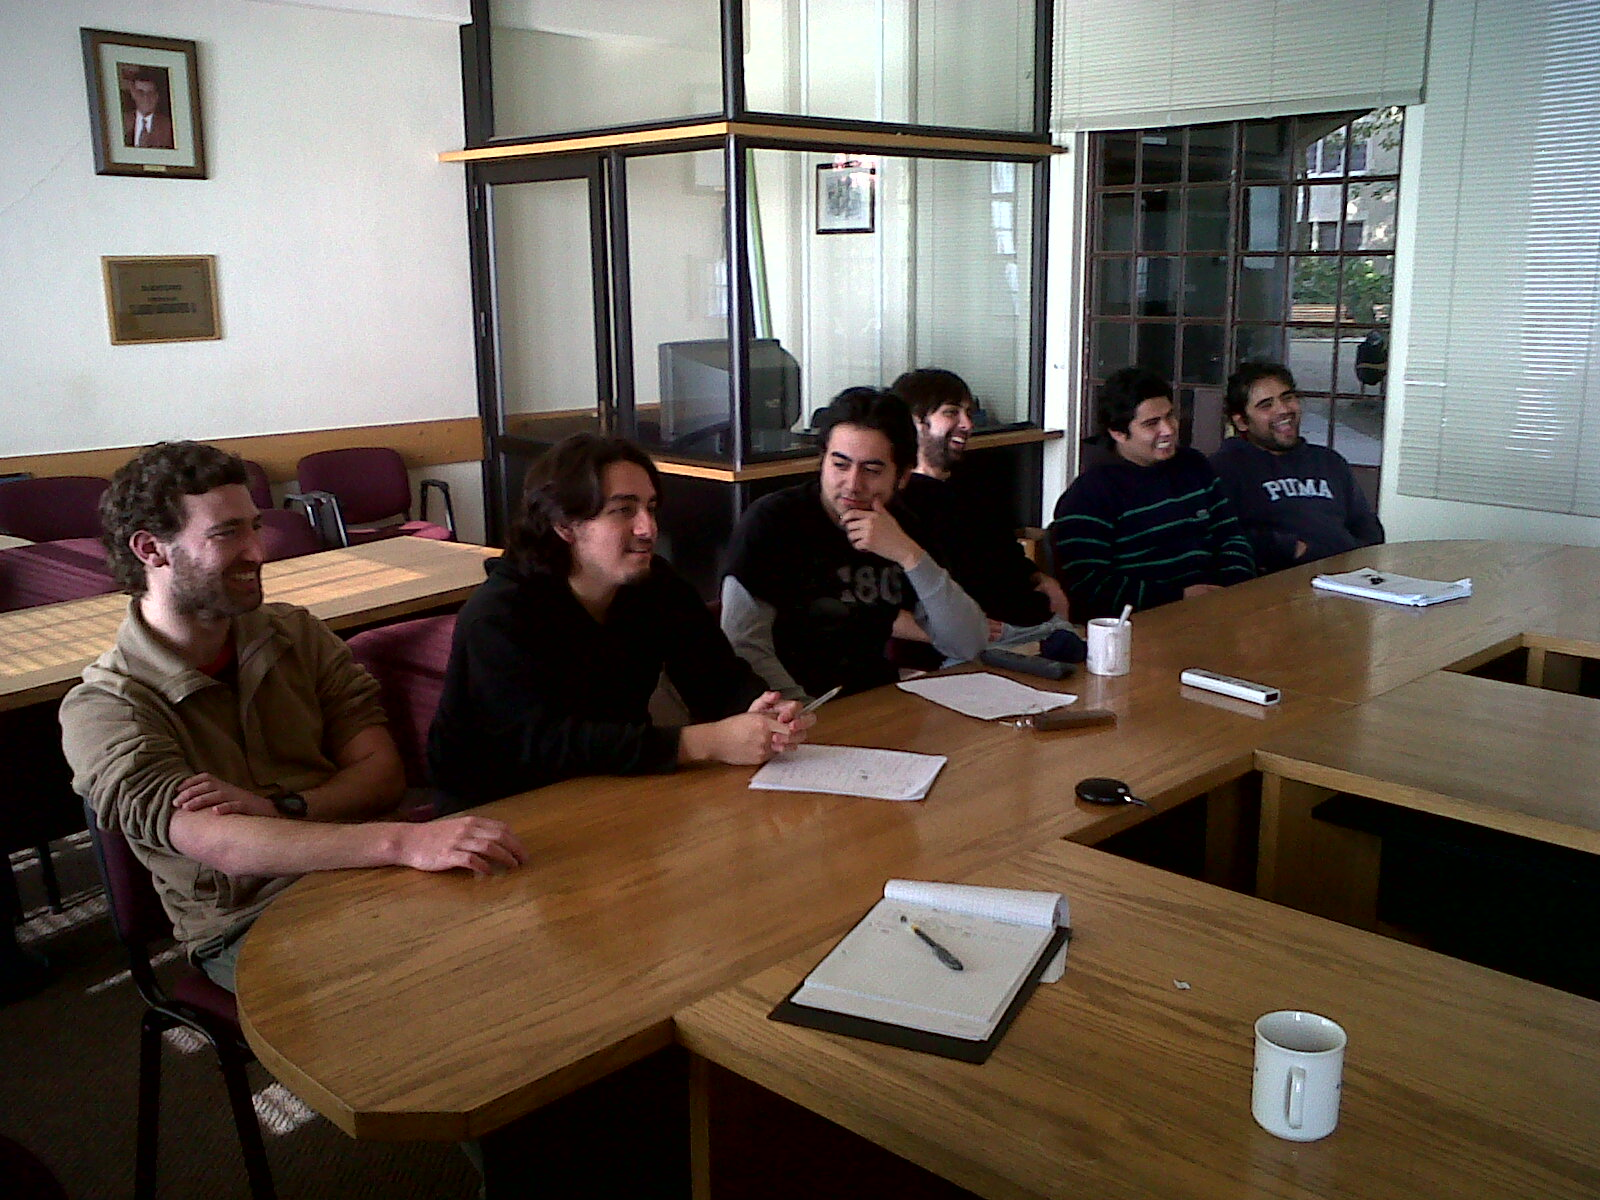
\includegraphics[width=0.8\textwidth]{images/leads1}\\\vspace{1cm}
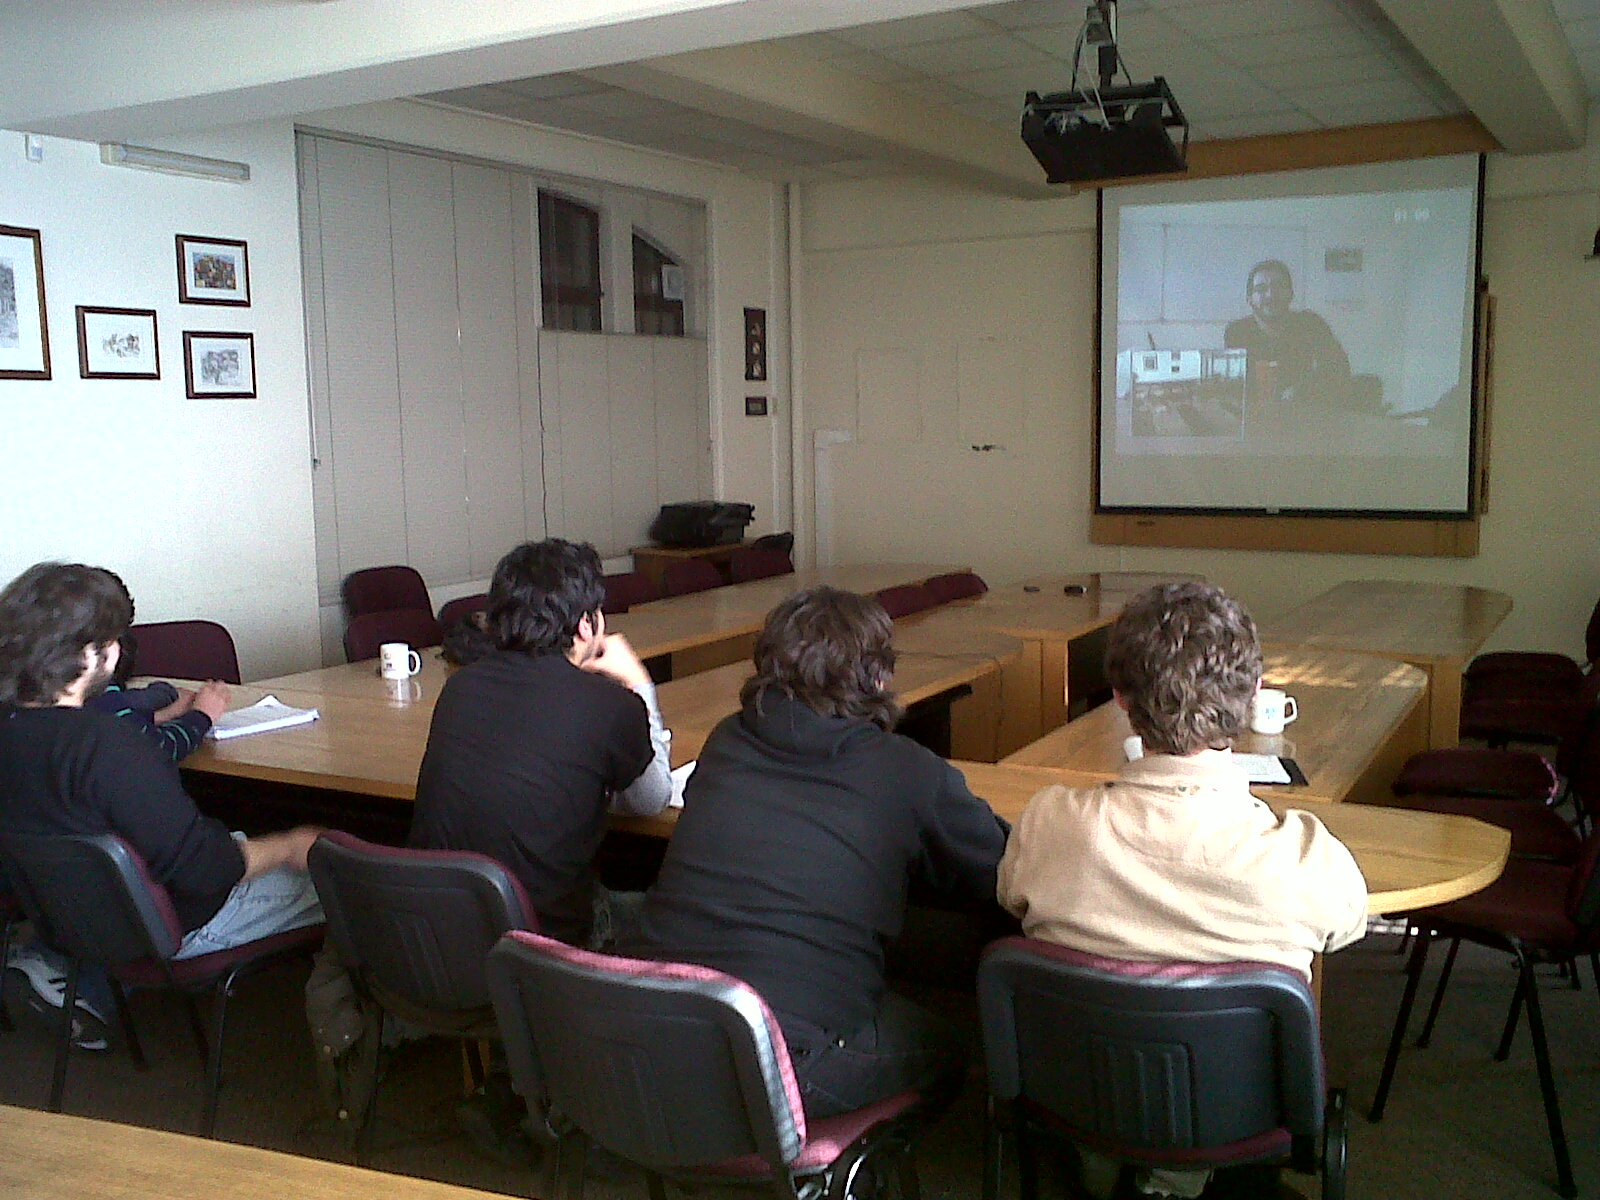
\includegraphics[width=0.8\textwidth]{images/leads2}
\end{center}
% CORRECCION &

\newpage
\subsection{Minutas de reuniones}
\subsubsubsection{ACS Weekly Meeting}
\begin{verbatim}
ACS Weekly Phone Meeting 
Date: Monday, 2010-04-12 

Attendees: 
ESO: Bogdan, Gianluca, Heiko, JosephSchwarz, 
NRAO: ArneGrimstrup, JorgeAvarias 
JSI: 
AOT: 
ALMA Chile: Ale 
UTFSM: GabrielZamora CristianMaureira 

Control contact number: +1-203-607-6471 (Passcode 203403#) 

General issues 

Alma has a promising candidate for a new board to replace the VMEs with 64 
bit architecture, to support more memory. Details from Thomas J. 
All module owners please fix their tests on 8.2 branch and HEAD. 

Ale Caproni 

Last week: 

CONTROL: Some issues with TotalPower testing, also due to STEs gotten messed up 
by other testers. 
The TP component has been changed to use the C++ API of the Bulk data libs, 
without reusing the IDL wrapper of the bulk data component. This works fine 
now, but still would like to discuss changes to the BD IDL for the long term. 
Will be at ESO early May. Things to be discussed should be added to Ale's 
Main.May2010 page.

Arne Grimstrup 

Last week: 

Continued investigation of COMP-3072 (with J. Avarias) 
problem still occurs with RHEL 5.4 version of CASA 
select is monitoring a bad file descriptor which triggers an exception 
in the TAO code. Telecon with UTFSM regarding future projects 
(with G. Chiozzi, H. Sommer, et. al.) Support 
Investigation of 64-bit test faults in NRI (H. Sommer)(with J. Avarias) 
Template method was invoking unsigned long version of getValue method 
that didn't exist Documentation for generated Python bindings (J. Kern) 
Questions regarding Python Binding Generator (J. Kern) 
Problem building ACS in INTROOT (J. Avarias) 

This week: 
Continue work on COMP-3072 
Continue work on COMP-830 

Bogdan Jeram 

Last week: 
Monday public holiday 
4 days of vacation 

Heiko Sommer 

Last week: 

Worked out HibernateDAL's usage of Archive's new archiveConfig.properties 
mechanism, together with Holger. 
Finalized 8.1 CVS logs and release notes. Pre-release of 9.0 VM. 
Discussions, e.g. TP with Ale and others 
Support, e.g. XSD validation, CDB performance fix, manager error messages, 
1 day leave 
Telecon with UTFSM about current projects 
quarterly report for ESO 

Helmut Tischer 

Last week: 
Vacation 

This week: 
COMP-2214 continuing 

Joe Schwarz 

Last week: 

Discussed problem of simultaneous use of SB by > 1 STE; change in 
lifecycle-handling needed 
Reviewed FP6 quarterly report from U. of Cambridge 
Worked on Total Power crash of Java container; suggested JNI 
debugging options for JVM runtime to Jeff and Ville, also removing
 native method invocation from class constructor (this didn't 
make any difference, however); got help from Roberto, who looked 
at logs and said he saw no bulk data issues 
Discussed CDR8 preparations w/Heiko 
Tried (and failed) to convince Brian to take Observation Control 
(not yet delivered) out of R7.1 
One day's leave 

This week: 
CDR8 preparation, ACS 9.0 planning 
Continue investigation of Total Power problem 
Return to classpath generation 

Jorge Avarias 

Last week: 

COMP-3749: ACS to introduce a new log level between DEBUG and TRACE 
Finished to make the last changes to the tests (Changed ACS_LOG_STDOUT 
from 2 to 1 new trace) 
All the tests affected by this are passing. 
Continued investigation of COMP-3072 (with A, Grimstrup) 
Fixed NRI ACS 64 bits building problems: 
The method unsigned long cdb::DAONode::getValue(char const*) 
was missing. probably some code is using unsigned long instead 
CORBA::ULong (in 32 bits they have the same length, in 64 they have not) 
Support: 
CONTROL/ACC/cppContainer crash (T. Powers) 
CONTROL/ACC/javaContainer crash, JVM is crashing with Seg. Fault 
(J. Kern, V. Suoranta) 
Problems building ACS in INTROOT (ACS is already built in ACSROOT) 
(S. Rankin) 


Matej Sekoranja 

Last week: 
HibernateDAL now skips loading all .dtd files, XMLSchema.xsd and xml.xsd so 
that Oracle's XMLTYPE checks don't get confused. 

This week: 
At CERN, but available for emergency ACS work. 

This week: 
TMCDB integration at the OSF 

UTFSM 

Last week: 

DDS Logging Service 
All the main goals are completed 
There are one pending task, write a "state of art" in this topic, for the paper 
accepted in the SPIE Meeting with people at ESO to define project objectives. 
Planning
Python support for BACI Properties 
ACS Code Generation 
ACS Windows Porting (Rodrigo and Heiko to integrate Java porting, Camillo and 
Gianluca to continue with C++ porting)
\end{verbatim}
\newpage
\subsubsubsection{OSF Coordination Meeting}

\begin{verbatim}
Date: Tue, 2010-05-18, 11:00 Chile, 9:00 Socorro, 17:00 Germany 
Attendees: 

ALMA-Chile: MatiasMora 
NRAO-Socorro: JorgeAvarias 
ESO-Garching: HeikoSommers 
UTFSM: GabrielZamora, TomasStaig, ArturoHoffstadt, CristianMaureira 
UCN: JaimePavlich 

Contact Info 
When: 11:00 Chile / 9:00 NM / 17:00 Germany 
Chile (toll free): 800532833 
International: +1 3032480281 
Access Code: 4676238 
Web Conferencing URL: http://net.globalcrossing.com/conferencing/ 

Agenda 
ALMA-CONICYT #31090034 (UTFSM) 
Projects 
ACS Windows Porting: The first version of the gcc-wrapper (gcc -> cl) is 
ready, we need to test with real examples to improve it. 
Code Generation: Luigi sent us a project proposal. Because Luigi was on
 vacations the last week, the meeting for this project is pending 
Alarms Configuration GUI: 
The project is ready, but there are some details with the redaction. 
Rules view that Tomas will fix in the week. 
Cristian Maureira and Tomas Staig will work on the documentation the 
next week. 
Official acceptance by ACS. 
Sampling System GUI: 
Juan Reyes and Cristian Maureira closed two of the three pending bugs, 
there are only one pending, that will be ready during the week. 
Official acceptance by ACS. 
ALMA-CONICYT #31080031 (AIA) 
Teams working on papers and on a new task about implementing TSP with 
their paper techniques 
HPC must to define the input framework and do some testing with TSP 
SebastianDuran and WalterFarina will be helping MatiasMora on what 
he needs for his thesis 
Second class this week Valpo. and next week Stgo. about advanced 
AI techniques 
Looking for possibilities of collaborations with MAIA-INRIA 
Summer Jobs 2010 
Pending reports! 
UCN Current Status 
Mini-ACS-Workshop from April 27th to May 10th. Funded by 
ALMA #31090026. 
Repository for UCN projects: http://goos-acs.googlecode.com 
gCCD status 
Implementing support for SBIG cameras 
Moving configuration to CDB 
gDome status 
gDome group are new students. After several intensive sessions 
they created the first version of the Dome component. 
Documentation: installation and system manuals. 
Misc 
ACS Scientific Linux distribution mirror repo here at UTFSM (ArturoHoffstadt).
\end{verbatim}


\end{document}
